\INEchaptercarta{Niñez que labora y su escolaridad}{}



\cajita{Tasa de trabajo infantil}{El trabajo infantil suele interferir con el proceso educativo de un niño, es por esto que es importante conocer que porcentaje de los niños trabajan. Para el 2014 la tasa de trabajo infantil se ubico en 10.7\%, esto es, 1.2 puntos más que en 2013, pero 8.7 puntos menos que en 2012.}{Tasa de la población menor a 14 años que realiza actividades económicas}{República de Guatemala, serie histórica, en porcentaje}{\ \\[0mm]\begin{tikzpicture}[x=1pt,y=1pt]  % Created by tikzDevice version 0.9 on 2016-02-28 17:18:14
% !TEX encoding = UTF-8 Unicode
\definecolor{fillColor}{RGB}{255,255,255}
\path[use as bounding box,fill=fillColor,fill opacity=0.00] (0,0) rectangle (289.08,198.74);
\begin{scope}
\path[clip] (  0.00,  0.00) rectangle (289.08,198.74);

\path[] (  0.00,  0.00) rectangle (289.08,198.74);
\end{scope}
\begin{scope}
\path[clip] (  0.00,  0.00) rectangle (289.08,198.74);

\path[] ( -0.52, 15.61) rectangle (280.54,191.48);

\path[] (  0.00, 44.24) --
	(280.54, 44.24);

\path[] (  0.00, 85.51) --
	(280.54, 85.51);

\path[] (  0.00,126.79) --
	(280.54,126.79);

\path[] (  0.00,168.06) --
	(280.54,168.06);

\path[] (  0.00, 23.61) --
	(280.54, 23.61);

\path[] (  0.00, 64.88) --
	(280.54, 64.88);

\path[] (  0.00,106.15) --
	(280.54,106.15);

\path[] (  0.00,147.42) --
	(280.54,147.42);

\path[] (  0.00,188.70) --
	(280.54,188.70);

\path[] ( 52.18, 15.61) --
	( 52.18,191.48);

\path[] (140.01, 15.61) --
	(140.01,191.48);

\path[] (227.84, 15.61) --
	(227.84,191.48);
\definecolor{drawColor}{RGB}{0,0,255}

\path[draw=drawColor,line width= 1.7pt,line join=round] ( 52.18,183.49) --
	(140.01,101.65) --
	(227.84,112.01);
\definecolor{drawColor}{RGB}{0,0,0}

\node[text=drawColor,anchor=base,inner sep=0pt, outer sep=0pt, scale=  1.02] at ( 52.18,187.46) {19.4};

\node[text=drawColor,anchor=base,inner sep=0pt, outer sep=0pt, scale=  1.02] at (140.01, 89.74) {9.5};

\node[text=drawColor,anchor=base,inner sep=0pt, outer sep=0pt, scale=  1.02] at (227.84,115.98) {10.7};

\path[draw=drawColor,line width= 0.1pt,line join=round] (  0.00, 23.61) -- (280.54, 23.61);

\path[] ( -0.52, 15.61) rectangle (280.54,191.48);
\end{scope}
\begin{scope}
\path[clip] (  0.00,  0.00) rectangle (289.08,198.74);

\path[] (  0.00, 15.61) --
	(280.54, 15.61);
\end{scope}
\begin{scope}
\path[clip] (  0.00,  0.00) rectangle (289.08,198.74);

\path[] ( 52.18, 12.86) --
	( 52.18, 15.61);

\path[] (140.01, 12.86) --
	(140.01, 15.61);

\path[] (227.84, 12.86) --
	(227.84, 15.61);
\end{scope}
\begin{scope}
\path[clip] (  0.00,  0.00) rectangle (289.08,198.74);
\definecolor{drawColor}{RGB}{0,0,0}

\node[text=drawColor,anchor=base,inner sep=0pt, outer sep=0pt, scale=  1.00] at ( 52.18,  2.85) {2012};

\node[text=drawColor,anchor=base,inner sep=0pt, outer sep=0pt, scale=  1.00] at (140.01,  2.85) {2013};

\node[text=drawColor,anchor=base,inner sep=0pt, outer sep=0pt, scale=  1.00] at (227.84,  2.85) {2014};
\end{scope}
  \end{tikzpicture} }{Instituto Nacional de Estadística, con datos de ENEI II-2014}



\cajita{Tasa de trabajo infantil por sexo}{El trabajo infantil se presenta en mayor proporción en niños que en niñas, con una diferencia en puntos porcentuales de 8.3}{Tasa de la población menor a 14 años que realiza actividades económicas según sexo}{República de Guatemala, año 2014, en porcentaje}{\ \\[0mm]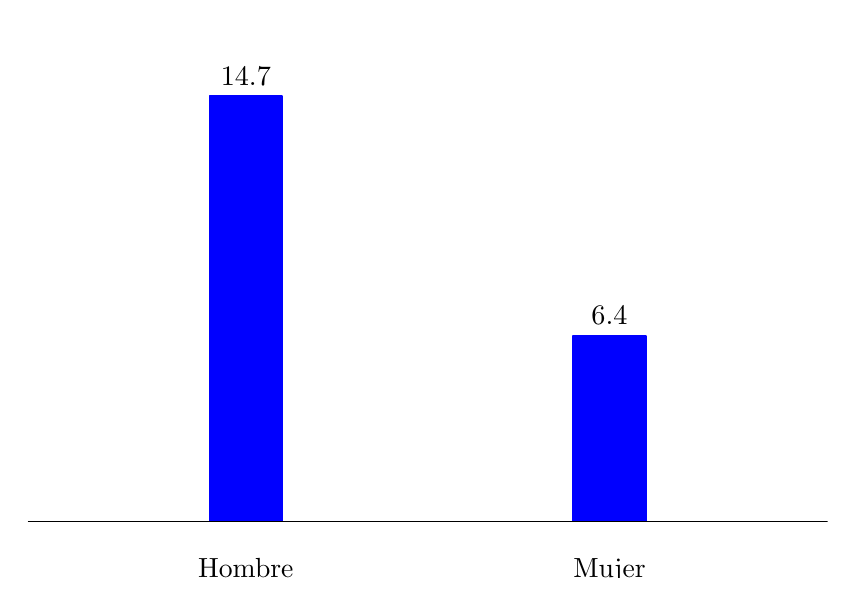
\begin{tikzpicture}[x=1pt,y=1pt]  % Created by tikzDevice version 0.9 on 2016-02-28 17:19:38
% !TEX encoding = UTF-8 Unicode
\definecolor{fillColor}{RGB}{255,255,255}
\path[use as bounding box,fill=fillColor,fill opacity=0.00] (0,0) rectangle (289.08,198.74);
\begin{scope}
\path[clip] (  0.00,  0.00) rectangle (289.08,198.74);

\path[] (  0.00,  0.00) rectangle (289.08,198.74);
\end{scope}
\begin{scope}
\path[clip] (  0.00,  0.00) rectangle (289.08,198.74);

\path[] (  0.00, 12.77) rectangle (289.08,181.67);

\path[] ( 78.84, 12.77) --
	( 78.84,181.67);

\path[] (210.24, 12.77) --
	(210.24,181.67);
\definecolor{drawColor}{RGB}{0,0,255}
\definecolor{fillColor}{RGB}{0,0,255}

\path[draw=drawColor,line width= 0.6pt,line join=round,fill=fillColor] ( 65.70, 20.44) rectangle ( 91.98,173.99);

\path[draw=drawColor,line width= 0.6pt,line join=round,fill=fillColor] (197.10, 20.44) rectangle (223.38, 87.36);
\definecolor{drawColor}{RGB}{0,0,0}

\path[draw=drawColor,line width= 0.1pt,line join=round] (  0.00, 20.44) -- (289.08, 20.44);

\node[text=drawColor,anchor=base,inner sep=0pt, outer sep=0pt, scale=  1.02] at ( 78.84,177.96) {14.7};

\node[text=drawColor,anchor=base,inner sep=0pt, outer sep=0pt, scale=  1.02] at (210.24, 91.33) {6.4};

\path[] (  0.00, 12.77) rectangle (289.08,181.67);
\end{scope}
\begin{scope}
\path[clip] (  0.00,  0.00) rectangle (289.08,198.74);

\path[] (  0.00, 12.77) --
	(289.08, 12.77);
\end{scope}
\begin{scope}
\path[clip] (  0.00,  0.00) rectangle (289.08,198.74);

\path[] ( 78.84, 10.02) --
	( 78.84, 12.77);

\path[] (210.24, 10.02) --
	(210.24, 12.77);
\end{scope}
\begin{scope}
\path[clip] (  0.00,  0.00) rectangle (289.08,198.74);
\definecolor{drawColor}{RGB}{0,0,0}

\node[text=drawColor,anchor=base,inner sep=0pt, outer sep=0pt, scale=  1.00] at ( 78.84, -0.00) {Hombre};

\node[text=drawColor,anchor=base,inner sep=0pt, outer sep=0pt, scale=  1.00] at (210.24, -0.00) {Mujer};
\end{scope}
  \end{tikzpicture} }{Instituto Nacional de Estadística, con datos de ENEI II-2014}


\cajita{Trabajo infantil y pea por dominio de estudio}{Al desagregar la información por dominio de estudio se puede apreciar que los niños del área rural nacional tienen mayor incidencia en la tasa de trabajo infantil, mientras que este indicador disminuye para los los niños en el área urbano metropolitano, donde el 4.4\% de los niños trabajan.}{Proporción de la población menor a 14 años que realiza actividades económicas, por dominio de estudio}{República de Guatemala, año 2014, en porcentaje}{\ \\[0mm]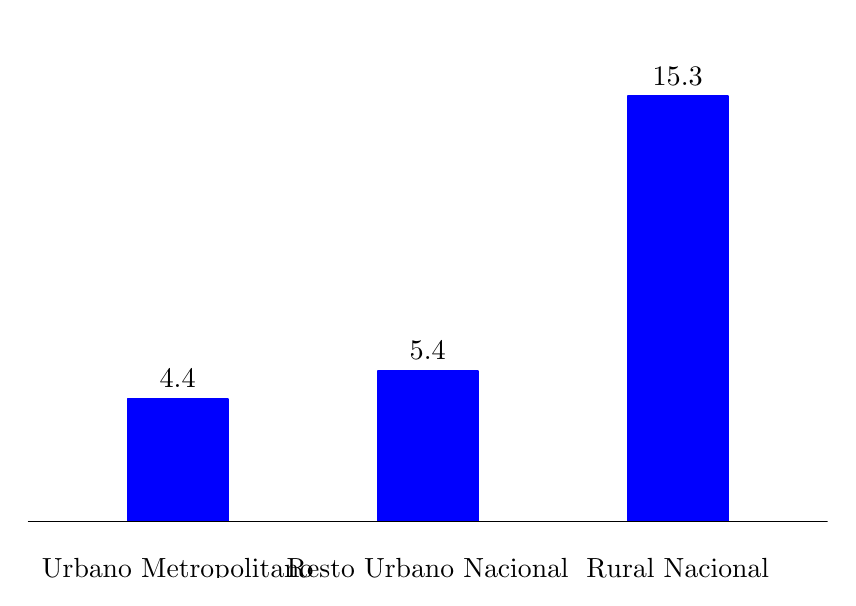
\begin{tikzpicture}[x=1pt,y=1pt]  % Created by tikzDevice version 0.9 on 2016-02-28 17:18:16
% !TEX encoding = UTF-8 Unicode
\definecolor{fillColor}{RGB}{255,255,255}
\path[use as bounding box,fill=fillColor,fill opacity=0.00] (0,0) rectangle (289.08,198.74);
\begin{scope}
\path[clip] (  0.00,  0.00) rectangle (289.08,198.74);

\path[] (  0.00,  0.00) rectangle (289.08,198.74);
\end{scope}
\begin{scope}
\path[clip] (  0.00,  0.00) rectangle (289.08,198.74);

\path[] (  0.00, 12.77) rectangle (289.08,181.67);

\path[] ( 54.20, 12.77) --
	( 54.20,181.67);

\path[] (144.54, 12.77) --
	(144.54,181.67);

\path[] (234.88, 12.77) --
	(234.88,181.67);
\definecolor{drawColor}{RGB}{0,0,255}
\definecolor{fillColor}{RGB}{0,0,255}

\path[draw=drawColor,line width= 0.6pt,line join=round,fill=fillColor] ( 36.13, 20.44) rectangle ( 72.27, 64.65);

\path[draw=drawColor,line width= 0.6pt,line join=round,fill=fillColor] (126.47, 20.44) rectangle (162.61, 74.69);

\path[draw=drawColor,line width= 0.6pt,line join=round,fill=fillColor] (216.81, 20.44) rectangle (252.95,173.99);
\definecolor{drawColor}{RGB}{0,0,0}

\path[draw=drawColor,line width= 0.1pt,line join=round] (  0.00, 20.44) -- (289.08, 20.44);

\node[text=drawColor,anchor=base,inner sep=0pt, outer sep=0pt, scale=  1.02] at ( 54.20, 68.62) {4.4};

\node[text=drawColor,anchor=base,inner sep=0pt, outer sep=0pt, scale=  1.02] at (144.54, 78.66) {5.4};

\node[text=drawColor,anchor=base,inner sep=0pt, outer sep=0pt, scale=  1.02] at (234.88,177.96) {15.3};

\path[] (  0.00, 12.77) rectangle (289.08,181.67);
\end{scope}
\begin{scope}
\path[clip] (  0.00,  0.00) rectangle (289.08,198.74);

\path[] (  0.00, 12.77) --
	(289.08, 12.77);
\end{scope}
\begin{scope}
\path[clip] (  0.00,  0.00) rectangle (289.08,198.74);

\path[] ( 54.20, 10.02) --
	( 54.20, 12.77);

\path[] (144.54, 10.02) --
	(144.54, 12.77);

\path[] (234.88, 10.02) --
	(234.88, 12.77);
\end{scope}
\begin{scope}
\path[clip] (  0.00,  0.00) rectangle (289.08,198.74);
\definecolor{drawColor}{RGB}{0,0,0}

\node[text=drawColor,anchor=base,inner sep=0pt, outer sep=0pt, scale=  1.00] at ( 54.20, -0.00) {Urbano Metropolitano};

\node[text=drawColor,anchor=base,inner sep=0pt, outer sep=0pt, scale=  1.00] at (144.54, -0.00) {Resto Urbano Nacional};

\node[text=drawColor,anchor=base,inner sep=0pt, outer sep=0pt, scale=  1.00] at (234.88, -0.00) {Rural Nacional};
\end{scope}
  \end{tikzpicture} }{Instituto Nacional de Estadística, con datos de ENEI II-2014}


\cajita{Trabajo infantil y escolaridad}{Es importante conocer el nivel de formación que tiene la niñez que realiza una tarea a cambio de una renumeración. Del total de los niños que están en primaria el 11.6\% trabaja, mientras que de los que están en básico el 12.1\% realiza tareas remuneradas. }{Proporción de la población menor a 14 años que realiza actividades económicas, por nivel de escolaridad}{República de Guatemala, año 2014, en porcentaje}{\ \\[0mm]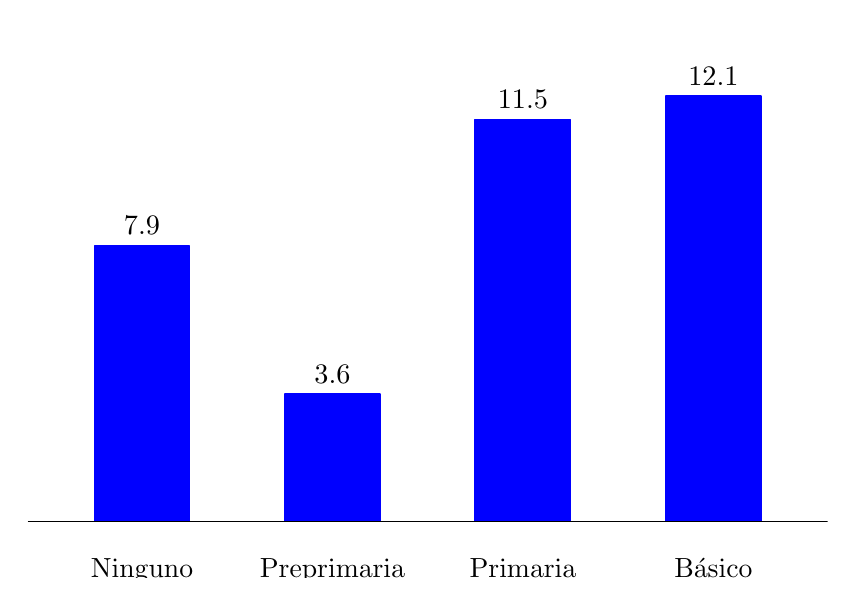
\begin{tikzpicture}[x=1pt,y=1pt]  % Created by tikzDevice version 0.9 on 2016-02-28 17:18:16
% !TEX encoding = UTF-8 Unicode
\definecolor{fillColor}{RGB}{255,255,255}
\path[use as bounding box,fill=fillColor,fill opacity=0.00] (0,0) rectangle (289.08,198.74);
\begin{scope}
\path[clip] (  0.00,  0.00) rectangle (289.08,198.74);

\path[] (  0.00,  0.00) rectangle (289.08,198.74);
\end{scope}
\begin{scope}
\path[clip] (  0.00,  0.00) rectangle (289.08,198.74);

\path[] (  0.00, 12.77) rectangle (289.08,181.67);

\path[] ( 41.30, 12.77) --
	( 41.30,181.67);

\path[] (110.13, 12.77) --
	(110.13,181.67);

\path[] (178.95, 12.77) --
	(178.95,181.67);

\path[] (247.78, 12.77) --
	(247.78,181.67);
\definecolor{drawColor}{RGB}{0,0,255}
\definecolor{fillColor}{RGB}{0,0,255}

\path[draw=drawColor,line width= 0.6pt,line join=round,fill=fillColor] ( 24.09, 20.44) rectangle ( 58.50,119.88);

\path[draw=drawColor,line width= 0.6pt,line join=round,fill=fillColor] ( 92.92, 20.44) rectangle (127.33, 66.30);

\path[draw=drawColor,line width= 0.6pt,line join=round,fill=fillColor] (161.75, 20.44) rectangle (196.16,165.52);

\path[draw=drawColor,line width= 0.6pt,line join=round,fill=fillColor] (230.58, 20.44) rectangle (264.99,173.99);
\definecolor{drawColor}{RGB}{0,0,0}

\path[draw=drawColor,line width= 0.1pt,line join=round] (  0.00, 20.44) -- (289.08, 20.44);

\node[text=drawColor,anchor=base,inner sep=0pt, outer sep=0pt, scale=  1.02] at ( 41.30,123.85) {7.9};

\node[text=drawColor,anchor=base,inner sep=0pt, outer sep=0pt, scale=  1.02] at (110.13, 70.27) {3.6};

\node[text=drawColor,anchor=base,inner sep=0pt, outer sep=0pt, scale=  1.02] at (178.95,169.49) {11.5};

\node[text=drawColor,anchor=base,inner sep=0pt, outer sep=0pt, scale=  1.02] at (247.78,177.96) {12.1};

\path[] (  0.00, 12.77) rectangle (289.08,181.67);
\end{scope}
\begin{scope}
\path[clip] (  0.00,  0.00) rectangle (289.08,198.74);

\path[] (  0.00, 12.77) --
	(289.08, 12.77);
\end{scope}
\begin{scope}
\path[clip] (  0.00,  0.00) rectangle (289.08,198.74);

\path[] ( 41.30, 10.02) --
	( 41.30, 12.77);

\path[] (110.13, 10.02) --
	(110.13, 12.77);

\path[] (178.95, 10.02) --
	(178.95, 12.77);

\path[] (247.78, 10.02) --
	(247.78, 12.77);
\end{scope}
\begin{scope}
\path[clip] (  0.00,  0.00) rectangle (289.08,198.74);
\definecolor{drawColor}{RGB}{0,0,0}

\node[text=drawColor,anchor=base,inner sep=0pt, outer sep=0pt, scale=  1.00] at ( 41.30, -0.00) {Ninguno};

\node[text=drawColor,anchor=base,inner sep=0pt, outer sep=0pt, scale=  1.00] at (110.13, -0.00) {Preprimaria};

\node[text=drawColor,anchor=base,inner sep=0pt, outer sep=0pt, scale=  1.00] at (178.95, -0.00) {Primaria};

\node[text=drawColor,anchor=base,inner sep=0pt, outer sep=0pt, scale=  1.00] at (247.78, -0.00) {Básico};
\end{scope}
  \end{tikzpicture} }{Instituto Nacional de Estadística, con datos de ENEI II-2014}


\cajita{Trabajo infantil, escolaridad y sexo}{Tanto para niños como para niñas la mayoría de la niñez que trabaja se encuentra estudiando la primaria o alcanzó algún grado de ella. }{Proporción de la población menor a 14 años que realiza actividades económicas, por nivel de escolaridad y sexo}{República de Guatemala, año 2014, en porcentaje}{\ \\[0mm]\begin{tikzpicture}[x=1pt,y=1pt]  % Created by tikzDevice version 0.9 on 2016-02-28 17:18:17
% !TEX encoding = UTF-8 Unicode
\definecolor{fillColor}{RGB}{255,255,255}
\path[use as bounding box,fill=fillColor,fill opacity=0.00] (0,0) rectangle (289.08,198.74);
\begin{scope}
\path[clip] (  0.00,  0.00) rectangle (289.08,198.74);

\path[] (  0.00,  0.00) rectangle (289.08,198.74);
\end{scope}
\begin{scope}
\path[clip] (  0.00,  0.00) rectangle (289.08,198.74);

\path[] (  0.00, 18.46) rectangle (289.08,172.85);

\path[] ( 41.30, 18.46) --
	( 41.30,172.85);

\path[] (110.13, 18.46) --
	(110.13,172.85);

\path[] (178.95, 18.46) --
	(178.95,172.85);

\path[] (247.78, 18.46) --
	(247.78,172.85);
\definecolor{drawColor}{RGB}{0,0,255}
\definecolor{fillColor}{RGB}{0,0,255}

\path[draw=drawColor,line width= 0.6pt,line join=round,fill=fillColor] ( 14.63, 18.46) rectangle ( 37.00, 28.36);
\definecolor{drawColor}{RGB}{157,187,255}
\definecolor{fillColor}{RGB}{157,187,255}

\path[draw=drawColor,line width= 0.6pt,line join=round,fill=fillColor] ( 45.60, 18.46) rectangle ( 67.97, 30.59);
\definecolor{drawColor}{RGB}{0,0,255}
\definecolor{fillColor}{RGB}{0,0,255}

\path[draw=drawColor,line width= 0.6pt,line join=round,fill=fillColor] ( 83.45, 18.46) rectangle (105.82, 20.55);
\definecolor{drawColor}{RGB}{157,187,255}
\definecolor{fillColor}{RGB}{157,187,255}

\path[draw=drawColor,line width= 0.6pt,line join=round,fill=fillColor] (114.43, 18.46) rectangle (136.80, 25.84);
\definecolor{drawColor}{RGB}{0,0,255}
\definecolor{fillColor}{RGB}{0,0,255}

\path[draw=drawColor,line width= 0.6pt,line join=round,fill=fillColor] (152.28, 18.46) rectangle (174.65,172.85);
\definecolor{drawColor}{RGB}{157,187,255}
\definecolor{fillColor}{RGB}{157,187,255}

\path[draw=drawColor,line width= 0.6pt,line join=round,fill=fillColor] (183.26, 18.46) rectangle (205.63,162.87);
\definecolor{drawColor}{RGB}{0,0,255}
\definecolor{fillColor}{RGB}{0,0,255}

\path[draw=drawColor,line width= 0.6pt,line join=round,fill=fillColor] (221.11, 18.46) rectangle (243.48, 32.49);
\definecolor{drawColor}{RGB}{157,187,255}
\definecolor{fillColor}{RGB}{157,187,255}

\path[draw=drawColor,line width= 0.6pt,line join=round,fill=fillColor] (252.08, 18.46) rectangle (274.45, 34.95);
\definecolor{drawColor}{RGB}{0,0,0}

\path[draw=drawColor,line width= 0.6pt,line join=round] (  0.00, 18.46) -- (289.08, 18.46);

\node[text=drawColor,anchor=base,inner sep=0pt, outer sep=0pt, scale=  0.83] at ( 25.81, 31.59) {5.5};

\node[text=drawColor,anchor=base,inner sep=0pt, outer sep=0pt, scale=  0.83] at ( 56.78, 33.82) {6.7};

\node[text=drawColor,anchor=base,inner sep=0pt, outer sep=0pt, scale=  0.83] at ( 94.64, 23.79) {1.2};

\node[text=drawColor,anchor=base,inner sep=0pt, outer sep=0pt, scale=  0.83] at (125.61, 29.07) {4.1};

\node[text=drawColor,anchor=base,inner sep=0pt, outer sep=0pt, scale=  0.83] at (163.47,176.08) {85.6};

\node[text=drawColor,anchor=base,inner sep=0pt, outer sep=0pt, scale=  0.83] at (194.44,166.10) {80.0};

\node[text=drawColor,anchor=base,inner sep=0pt, outer sep=0pt, scale=  0.83] at (232.30, 35.72) {7.8};

\node[text=drawColor,anchor=base,inner sep=0pt, outer sep=0pt, scale=  0.83] at (263.27, 38.18) {9.1};

\path[] (  0.00, 18.46) rectangle (289.08,172.85);
\end{scope}
\begin{scope}
\path[clip] (  0.00,  0.00) rectangle (289.08,198.74);

\path[] (  0.00, 18.46) --
	(289.08, 18.46);
\end{scope}
\begin{scope}
\path[clip] (  0.00,  0.00) rectangle (289.08,198.74);

\path[] ( 41.30, 15.71) --
	( 41.30, 18.46);

\path[] (110.13, 15.71) --
	(110.13, 18.46);

\path[] (178.95, 15.71) --
	(178.95, 18.46);

\path[] (247.78, 15.71) --
	(247.78, 18.46);
\end{scope}
\begin{scope}
\path[clip] (  0.00,  0.00) rectangle (289.08,198.74);
\definecolor{drawColor}{RGB}{0,0,0}

\node[text=drawColor,anchor=base,inner sep=0pt, outer sep=0pt, scale=  1.00] at ( 41.30,  5.69) {Ninguno};

\node[text=drawColor,anchor=base,inner sep=0pt, outer sep=0pt, scale=  1.00] at (110.13,  5.69) {Preprimaria};

\node[text=drawColor,anchor=base,inner sep=0pt, outer sep=0pt, scale=  1.00] at (178.95,  5.69) {Primaria};

\node[text=drawColor,anchor=base,inner sep=0pt, outer sep=0pt, scale=  1.00] at (247.78,  5.69) {Básico};
\end{scope}
\begin{scope}
\path[clip] (  0.00,  0.00) rectangle (289.08,198.74);
\coordinate (apoyo) at (55.98,189.21);
\coordinate (longitudFicticia) at (7.11,9.53);
\coordinate (longitud) at (7.11,7.11);
\coordinate (desX) at (142.21,0);
\coordinate (desY) at (0,1.21);
\definecolor[named]{ct1}{HTML}{
0000FF
}
\definecolor[named]{ct2}{HTML}{
9DBBFF
}
\definecolor[named]{ctb1}{HTML}{
0000FF
}
\definecolor[named]{ctb2}{HTML}{
9DBBFF
}
\path [fill=none] (apoyo) rectangle ($(apoyo)+(longitudFicticia)$)
node [xshift=0.3cm,inner sep=0pt, outer sep=0pt,midway,right,scale = 0.9]{Hombre};
\draw [color = ctb1,fill=ct1] ( $(apoyo)  + (desY) $) rectangle ($(apoyo)+ (desY) +(longitud)$);
\path [fill=none] ($(apoyo)+(desX)$) rectangle ($(apoyo)+(desX)+(longitudFicticia)$)
node [xshift=0.3cm,inner sep=0pt, outer sep=0pt,midway,right,scale = 0.9]{Mujer};
\draw [color = ctb2 ,fill=ct2] ( $(apoyo)  + (desY) + (desX) $) rectangle ($(apoyo)+ (desY)+ (desX) +(longitud)$);
\end{scope}
  \end{tikzpicture} }{Instituto Nacional de Estadística, con datos de ENEI II-2014}


\cajita{Trabajo infantil y escolaridad del jefe de hogar}{Es importante conocer el nivel educativo que tiene el jefe de hogar que manda a sus niños a realizar trabajos remunerados.
	
	 La mayoría de niños que realizan trabajo infantil viven en hogares donde el jefe de hogar apenas alcanzó algún nivel de la primaria, mientras que apenas un 0.2\% de los niños que trabajan provienen de hogares donde el jefe de hogar tiene un grado universitario. }{Distribución de la población menor a 14 años que realiza actividades económicas, por nivel de escolaridad del jefe de hogar}{República de Guatemala, año 2014, en porcentaje}{\ \\[0mm]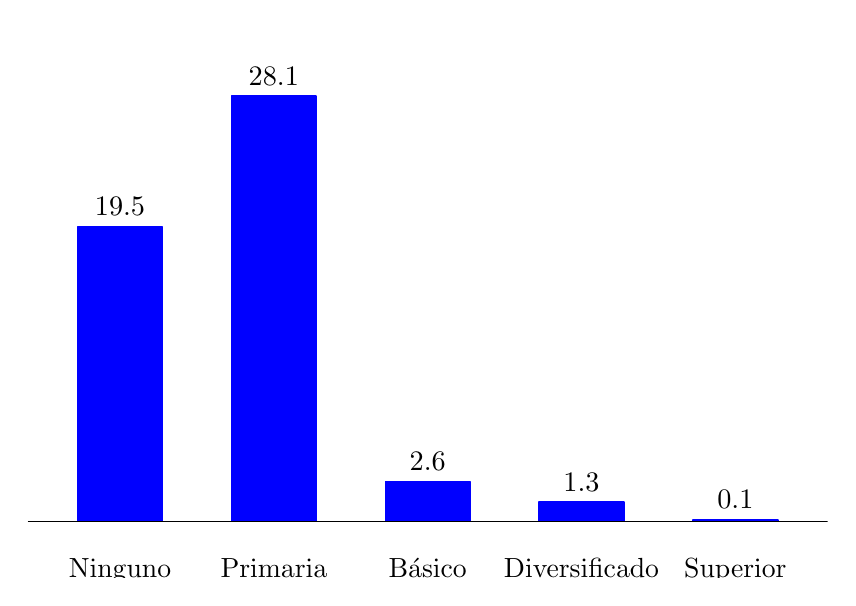
\begin{tikzpicture}[x=1pt,y=1pt]  % Created by tikzDevice version 0.9 on 2016-02-28 17:22:08
% !TEX encoding = UTF-8 Unicode
\definecolor{fillColor}{RGB}{255,255,255}
\path[use as bounding box,fill=fillColor,fill opacity=0.00] (0,0) rectangle (289.08,198.74);
\begin{scope}
\path[clip] (  0.00,  0.00) rectangle (289.08,198.74);

\path[] (  0.00,  0.00) rectangle (289.08,198.74);
\end{scope}
\begin{scope}
\path[clip] (  0.00,  0.00) rectangle (289.08,198.74);

\path[] (  0.00, 12.77) rectangle (289.08,181.67);

\path[] ( 33.36, 12.77) --
	( 33.36,181.67);

\path[] ( 88.95, 12.77) --
	( 88.95,181.67);

\path[] (144.54, 12.77) --
	(144.54,181.67);

\path[] (200.13, 12.77) --
	(200.13,181.67);

\path[] (255.72, 12.77) --
	(255.72,181.67);
\definecolor{drawColor}{RGB}{0,0,255}
\definecolor{fillColor}{RGB}{0,0,255}

\path[draw=drawColor,line width= 0.6pt,line join=round,fill=fillColor] ( 18.07, 20.44) rectangle ( 48.64,126.92);

\path[draw=drawColor,line width= 0.6pt,line join=round,fill=fillColor] ( 73.66, 20.44) rectangle (104.24,173.99);

\path[draw=drawColor,line width= 0.6pt,line join=round,fill=fillColor] (129.25, 20.44) rectangle (159.83, 34.69);

\path[draw=drawColor,line width= 0.6pt,line join=round,fill=fillColor] (184.84, 20.44) rectangle (215.42, 27.28);

\path[draw=drawColor,line width= 0.6pt,line join=round,fill=fillColor] (240.44, 20.44) rectangle (271.01, 20.94);
\definecolor{drawColor}{RGB}{0,0,0}

\path[draw=drawColor,line width= 0.1pt,line join=round] (  0.00, 20.44) -- (289.08, 20.44);

\node[text=drawColor,anchor=base,inner sep=0pt, outer sep=0pt, scale=  1.02] at ( 33.36,130.89) {19.5};

\node[text=drawColor,anchor=base,inner sep=0pt, outer sep=0pt, scale=  1.02] at ( 88.95,177.96) {28.1};

\node[text=drawColor,anchor=base,inner sep=0pt, outer sep=0pt, scale=  1.02] at (144.54, 38.66) {2.6};

\node[text=drawColor,anchor=base,inner sep=0pt, outer sep=0pt, scale=  1.02] at (200.13, 31.25) {1.3};

\node[text=drawColor,anchor=base,inner sep=0pt, outer sep=0pt, scale=  1.02] at (255.72, 24.91) {0.1};

\path[] (  0.00, 12.77) rectangle (289.08,181.67);
\end{scope}
\begin{scope}
\path[clip] (  0.00,  0.00) rectangle (289.08,198.74);

\path[] (  0.00, 12.77) --
	(289.08, 12.77);
\end{scope}
\begin{scope}
\path[clip] (  0.00,  0.00) rectangle (289.08,198.74);

\path[] ( 33.36, 10.02) --
	( 33.36, 12.77);

\path[] ( 88.95, 10.02) --
	( 88.95, 12.77);

\path[] (144.54, 10.02) --
	(144.54, 12.77);

\path[] (200.13, 10.02) --
	(200.13, 12.77);

\path[] (255.72, 10.02) --
	(255.72, 12.77);
\end{scope}
\begin{scope}
\path[clip] (  0.00,  0.00) rectangle (289.08,198.74);
\definecolor{drawColor}{RGB}{0,0,0}

\node[text=drawColor,anchor=base,inner sep=0pt, outer sep=0pt, scale=  1.00] at ( 33.36, -0.00) {Ninguno};

\node[text=drawColor,anchor=base,inner sep=0pt, outer sep=0pt, scale=  1.00] at ( 88.95, -0.00) {Primaria};

\node[text=drawColor,anchor=base,inner sep=0pt, outer sep=0pt, scale=  1.00] at (144.54, -0.00) {Básico};

\node[text=drawColor,anchor=base,inner sep=0pt, outer sep=0pt, scale=  1.00] at (200.13, -0.00) {Diversificado};

\node[text=drawColor,anchor=base,inner sep=0pt, outer sep=0pt, scale=  1.00] at (255.72, -0.00) {Superior};
\end{scope}
  \end{tikzpicture} }{Instituto Nacional de Estadística, con datos de ENEI II-2014}